% ******************************************************************	********************************************
%
% **************************************************************************************************************
\documentclass[ twoside,openright,titlepage,numbers=noenddot,%
				toc=bibliography,toc=listof,%
                footinclude=false,headinclude=false,cleardoublepage=empty,%
				BCOR=5mm,paper=a4,fontsize=11pt
                %,ngerman%
                ]{scrreprt}
%***************************************************************************************************************
% Note: Make all your adjustments in here
%***************************************************************************************************************
% ****************************************************************************************************
% htwsaar-i-mst-config.tex 
% ****************************************************************************************************  
\RequirePackage[utf8]{inputenc}				
 \DeclareUnicodeCharacter{00A0}{~}								
\RequirePackage[T1]{fontenc} 
								
% ****************************************************************************************************
% 1. Personal data and user ad-hoc commands
% ****************************************************************************************************
\newcommand{\myTitle}{Eine \LaTeX-Vorlage für Abschlussarbeiten im Bereich Informatik/Mechatronik-Sensortechnik (inkl. DFHI) an der htw saar}
\newcommand{\myDegree}{Bachelor of Science (B.\,Sc.)\xspace}
%\newcommand{\myDegree}{Master of Science (M.\,Sc.)\xspace}
\newcommand{\myDegreeType}{Bachelor\xspace}
%\newcommand{\myDegreeType}{Master\xspace}
\newcommand{\myDegreeCourse}{Praktische Informatik}
%\newcommand{\myDegreeCourse}{Informatik und Web-Engineering}
%\newcommand{\myDegreeCourse}{Kommunikationsinformatik}
%\newcommand{\myDegreeCourse}{Produktionsinformatik}
\newcommand{\myName}{Max Muster\xspace}
\newcommand{\myUni}{Hochschule für Technik und Wirtschaft des Saarlandes\xspace}
\newcommand{\myCompany}{SoftwareCenter Musterhausen\xspace}
\newcommand{\myFirstProf}{Prof. Dr.-Ing. André Miede\xspace}
\newcommand{\mySecondProf}{Prof. Dr. Thomas Kretschmer\xspace}
\newcommand{\myLocation}{Saarbrücken\xspace}
\newcommand{\myTime}{Tag.~Monat~Jahr\xspace}
\newcommand{\currentVersion}{Version 2.25, August 2024\xspace} % TODO: ggf. über git Versionsinformationen automatisch bereitstellen und verwenden

% ********************************************************************
% Setup, finetuning, and useful commands
% ********************************************************************
\newcounter{dummy} % necessary for correct hyperlinks (to index, bib, etc.)
% ****************************************************************************************************


% ****************************************************************************************************
% 2. Loading some handy packages
% ****************************************************************************************************
% ******************************************************************** 
% Packages with options that might require adjustments
% ******************************************************************** 
\PassOptionsToPackage{ngerman}{babel}   % change this to your language(s)
 \RequirePackage{babel}					
 \RequirePackage{csquotes}
	
\PassOptionsToPackage{language=auto,style=numeric-comp,backend=bibtex8,bibencoding=ascii,maxbibnames=50}{biblatex} % backend ggf. auf neueres Werkzeug (z.B. biber) anpassen
 \RequirePackage{biblatex}	
 %\bibliography{Bibliography}	% alter Befehl
 \addbibresource{Bibliography}

\PassOptionsToPackage{fleqn}{amsmath}		% math environments and more by the AMS 
 \RequirePackage{amsmath}

% ******************************************************************** 
% Setting up the page and margins
% ******************************************************************** 
\usepackage{geometry}
 \geometry{a4paper,left=25mm,right=35mm,top=25mm,bottom=30mm}
% DIESE WERTE SIND NICHT ZU VERÄNDERN -- DO NOT CHANGE THESE VALUES

% ******************************************************************** 
% General useful packages
% ******************************************************************** 
%\usepackage[automark]{scrpage2}
\PassOptionsToPackage{dvipsnames}{xcolor}
	\RequirePackage{xcolor} % [dvipsnames]  
	\definecolor{ingwi}{cmyk}{.9,0,0,0}
\usepackage{textcomp} % fix warning with missing font shapes
\usepackage{scrhack} % fix warnings when using KOMA with listings package          
\usepackage{xspace} % to get the spacing after macros right  
\usepackage{mparhack} % get marginpar right
%\usepackage{fixltx2e} % fixes some LaTeX stuff <-- ist seit 2015 nicht mehr notwendig
\PassOptionsToPackage{printonlyused}{acronym}
	\usepackage{acronym} % nice macros for handling all acronyms in the thesis
%\renewcommand{\bflabel}[1]{{#1}\hfill} % fix the list of acronyms
\usepackage{booktabs}
\usepackage{multirow}
\usepackage{todonotes} %Settings for ToDoNotes
% Eigene Shortcuts fuer laengere Befehle
	\newcommand{\todox}[1]{\todo[inline, size=\small]{#1}}
	%Nummerierte Anmerkungen
	\newcounter{todocounter}
	\renewcommand{\todox}[2][]{\stepcounter{todocounter}\todo[inline, size=\small,caption={\thetodocounter: #2}, #1]{\renewcommand{\baselinestretch}{0.5}\selectfont\thetodocounter: #2\par}}
\usepackage{blindtext}
%\usepackage{footmisc}
% ****************************************************************************************************


% ****************************************************************************************************
% 3. Setup floats: tables, (sub)figures, and captions
% ****************************************************************************************************
\usepackage{tabularx} % better tables
	\setlength{\extrarowheight}{3pt} % increase table row height
%\newcommand{\myfloatalign}{\centering} % to be used with each float for alignment
\usepackage{caption}
\captionsetup{format=hang,font=small}
\usepackage{subfig}
\usepackage{wrapfig}
% ****************************************************************************************************


% ****************************************************************************************************
% 6. Setup code listings
% ****************************************************************************************************
\usepackage{listings} 
%\lstset{emph={trueIndex,root},emphstyle=\color{BlueViolet}}%\underbar} % for special keywords
\lstset{language=[LaTeX]Tex,%C++,
    keywordstyle=\color{RoyalBlue},%\bfseries,
    basicstyle=\small\ttfamily,
    %identifierstyle=\color{NavyBlue},
    commentstyle=\color{Green}\ttfamily,
    stringstyle=\rmfamily,
    numbers=none,%left,%
    numberstyle=\scriptsize,%\tiny
    stepnumber=5,
    numbersep=8pt,
    showstringspaces=false,
    breaklines=true,
    frameround=ftff,
    frame=single,
		texcl=true,
    belowcaptionskip=.75\baselineskip
    %frame=L
} 
%Styles für verschiedene Sprachen festlegen, z.B. Java
\lstdefinestyle{Java}{
belowcaptionskip=1\baselineskip,
  breaklines=true,
  xleftmargin=\parindent,
  language=Java,
	texcl=true,
  showstringspaces=false,
  basicstyle=\footnotesize\ttfamily,
  keywordstyle=\bfseries\color{green!40!black},
  commentstyle=\itshape\color{purple!40!black},
  identifierstyle=\color{blue},
  stringstyle=\color{orange}}
% ****************************************************************************************************    		   


% ****************************************************************************************************
% 6. PDFLaTeX, hyperreferences and citation backreferences
% ****************************************************************************************************
% ********************************************************************
% Using PDFLaTeX
% ********************************************************************
\usepackage{xurl}  % better handling of long URLs / hyphenation
\PassOptionsToPackage{pdftex,hyperfootnotes=false,pdfpagelabels}{hyperref}
	\usepackage{hyperref}  % backref linktocpage pagebackref
\pdfcompresslevel=9
\pdfadjustspacing=1 
\PassOptionsToPackage{pdftex}{graphicx}
	\usepackage{graphicx} 
    

% ********************************************************************
% Hyperreferences
% ********************************************************************
\hypersetup{%
    %draft,	% = no hyperlinking at all (useful in b/w printouts)
    pdfstartpage=1, pdfstartview=Fit,%
	colorlinks=true, linktocpage=true,
	%urlcolor=Black, linkcolor=Black, citecolor=Black, %pagecolor=Black,%
	%urlcolor=brown, linkcolor=RoyalBlue, citecolor=green, %pagecolor=RoyalBlue,%
    % uncomment the following line if you want to have black links (e.g., for printing)
    colorlinks=false, pdfborder={0 0 0},
    breaklinks=true, pdfpagemode=UseNone, pageanchor=true, pdfpagemode=UseOutlines,%
    plainpages=false, bookmarksnumbered, bookmarksopen=true, bookmarksopenlevel=1,%
    hypertexnames=true, pdfhighlight=/O,%nesting=true,%frenchlinks,%
    pdftitle={\myTitle},%
    pdfauthor={\textcopyright\ \myName, \myUni},%
    pdfsubject={},%
    pdfkeywords={},%
    pdfcreator={pdfLaTeX},%
    pdfproducer={LaTeX with hyperref}%
}   

% ********************************************************************
% Setup autoreferences
% ********************************************************************
% There are some issues regarding autorefnames
% http://www.ureader.de/msg/136221647.aspx
% http://www.tex.ac.uk/cgi-bin/texfaq2html?label=latexwords
% you have to redefine the makros for the 
% language you use, e.g., american, ngerman
% (as chosen when loading babel/AtBeginDocument)
% ********************************************************************
\makeatletter
\@ifpackageloaded{babel}%
    {%
       \addto\extrasamerican{%
					\renewcommand*{\figureautorefname}{Figure}%
					\renewcommand*{\tableautorefname}{Table}%
					\renewcommand*{\partautorefname}{Part}%
					\renewcommand*{\chapterautorefname}{Chapter}%
					\renewcommand*{\sectionautorefname}{Section}%
					\renewcommand*{\subsectionautorefname}{Section}%
					\renewcommand*{\subsubsectionautorefname}{Section}% 	
				}%
       \addto\extrasngerman{% 
					\renewcommand*{\chapterautorefname}{Kapitel}%
					\renewcommand*{\sectionautorefname}{Abschnitt}%
					\renewcommand*{\subsectionautorefname}{Abschnitt}%
					\renewcommand*{\subsubsectionautorefname}{Abschnitt}% 
					\renewcommand*{\paragraphautorefname}{Absatz}%
					\renewcommand*{\subparagraphautorefname}{Absatz}%
					\renewcommand*{\footnoteautorefname}{Fußnote}%
					\renewcommand*{\FancyVerbLineautorefname}{Zeile}%
					\renewcommand*{\theoremautorefname}{Theorem}%
					\renewcommand*{\appendixautorefname}{Anhang}%
					\renewcommand*{\equationautorefname}{Gleichung}%        
					\renewcommand*{\itemautorefname}{Punkt}%
				}%	
			% Fix to getting autorefs for subfigures right (thanks to Belinda Vogt for changing the definition)
			\providecommand{\subfigureautorefname}{\figureautorefname}%  			
    }{\relax}
\makeatother


% ****************************************************************************************************
% 6. Last calls before the bar closes
% ****************************************************************************************************
% ********************************************************************
% Development Stuff
% ********************************************************************
%\listfiles
\PassOptionsToPackage{l2tabu,orthodox,abort}{nag}
	\usepackage{nag}
%\PassOptionsToPackage{warning, all}{onlyamsmath}
%	\usepackage{onlyamsmath}


% ****************************************************************************************************
% 7. Further adjustments (experimental)
% ****************************************************************************************************
%\usepackage{tocbibind} %Allows us to add Bibliography to ToC
\usepackage{enumitem}
\setdescription{font=\normalfont\bfseries} %Changes the appearance of description items
\usepackage[activate={true,nocompatibility},final,tracking=true,kerning=true,spacing=true,factor=1100,stretch=10,shrink=10]{microtype}


% ********************************************************************
% Using different fonts
% ********************************************************************
%\usepackage{lmodern} % <-- no osf support :-(
%\usepackage[tt=false]{libertine} % [osf]
%\usepackage{luximono} 
%\usepackage[urw-garamond]{mathdesign} <-- no osf support :-(
\usepackage{mathpazo} 
%\usepackage{libertinus} % math? osf?

\setkomafont{disposition}{\bfseries}
% ****************************************************************************************************

%********************************************************************
% Hyphenation
%*******************************************************
%\hyphenation{put special hyphenation here}

% ********************************************************************
% GO!GO!GO! MOVE IT!
%*******************************************************
\begin{document}
\frenchspacing
\raggedbottom
\selectlanguage{ngerman} % american ngerman
\pagenumbering{roman}
\pagestyle{plain}
%*******************************************************
% Frontmatter
%*******************************************************
%*******************************************************
% Titlepage
% [Nicht zu verändern]
%*******************************************************
\begin{titlepage}\linespread{1.5}\selectfont

\includegraphics[width=\linewidth]{Graphics/htwsaar_Logo_inwi_head_VF_4C_crop}
  \begin{center}
    \large  
    \hfill
    \vfill
    \begingroup
      \Large\bfseries Ausarbeitung 
    \endgroup
		
		\bigskip
		
    zum Thema Lambda-Architektur \\
    im Rahmen des Kurses Software-Architektur \\
    an der \myUni \\
    
  \vfill
	
  \begingroup
    \Large\bfseries\myTitle 
  \endgroup
	
	\bigskip
	
  vorgelegt von \\
  Tobias Kronser \\
  Moritz Schönenberger \\
  Leon Weyand \\
	
  \vfill
	
  betreut und begutachtet von \\
  \myFirstProf 
	
  \vfill
	
  \myLocation, \myTime                   

    \end{center}       
\end{titlepage}   
%%*******************************************************
% Titlepage
% [Nicht zu verändern]
%*******************************************************
\begin{titlepage}\linespread{1.5}\selectfont
\noindent
\includegraphics[width=3cm]{Graphics/logo-dfhi} \hfill 
\includegraphics[width=3cm]{Graphics/logo-uni-de-lorraine} \medskip

\noindent
\includegraphics[width=\linewidth]{Graphics/htwsaar_Logo_inwi_head_VF_4C_crop}

  \begin{center}
    \large  
    \hfill
    \vfill
    \begingroup
      \Large\bfseries\myDegreeType-Thesis 
    \endgroup
		
	\bigskip
		
    zur Erlangung des akademischen Grades \\
    \myDegree \\ 
    an der \myUni \\
	und \\
	der Université de Lorraine, Metz \\ 
    im Studiengang \myDegreeCourse \\
    des Deutsch-Französischen Hochschulinstituts (DFHI / ISFATES) \\ 
    
  \vfill
	
  \begingroup
    \Large\bfseries\myTitle 
  \endgroup
	
	\bigskip
	
  vorgelegt von \\
  \myName
	
  \vfill
	
  betreut und begutachtet von \\
  \myFirstProf \\
  \mySecondProf 
	
  \vfill
	
  \myLocation, \myTime                   

    \end{center}       
\end{titlepage}    % <-- für DFHI-Studiengänge
\cleardoublepage%*******************************************************
% Declaration
% [Nicht übersetzen, 
% weil Prüfungsleistung an dt. Hochschule]
%*******************************************************
\pdfbookmark[0]{Selbständigkeitserklärung}{declaration}
\chapter*{Selbständigkeitserklärung}
%\thispagestyle{empty}

Ich versichere, dass ich die vorliegende Arbeit (bei einer Gruppenarbeit: den entsprechend gekennzeichneten
Anteil der Arbeit) selbständig verfasst und keine anderen als die angegebenen Quellen und
Hilfsmittel benutzt habe.

Ich erkläre hiermit weiterhin, dass die vorgelegte Arbeit zuvor weder von mir noch von einer anderen Person an dieser oder einer
anderen Hochschule eingereicht wurde.

Darüber hinaus ist mir bekannt, dass die Unrichtigkeit dieser Erklärung eine Benotung der 
Arbeit mit der Note "`nicht ausreichend"' zur Folge hat und einen Ausschluss von der Erbringung 
weiterer Prüfungsleistungen zur Folge haben kann.
\bigskip
 
\noindent\textit{\myLocation, \myTime}

\smallskip

\begin{flushright}
    \begin{tabular}{m{5cm}}
        \\ \hline
        \centering\myName \\
    \end{tabular}
\end{flushright}
%\cleardoublepage%*******************************************************
% Sperrvermerk 
% [Nicht übersetzen, 
% weil Prüfungsleistung an dt. Hochschule]
%*******************************************************
% Der Sperrvermerk kann entfernt werden, wenn die Arbeit z.B. nicht im 
% Zusammenarbeit mit einem Unternehmen angefertigt wurde oder kein
% Sperrvermerk verlangt wird.

\pdfbookmark[0]{Sperrvermerk}{sperrvermerk}
\chapter*{Sperrvermerk}
%\thispagestyle{empty}

Die vorliegende Arbeit mit dem Titel "`\myTitle"' enthält vertrauliche Daten des Unternehmens \myCompany.

Die Arbeit darf nur dem Erst- und Zweitgutachter sowie befugten Mitgliedern des Prüfungsausschusses zugänglich gemacht werden. 
Eine Veröffentlichung und Vervielfältigung der Arbeit ist -- auch in Auszügen -- nicht gestattet.

Eine Einsichtnahme der Arbeit durch Unbefugte bedarf einer ausdrücklichen Genehmigung des Verfassers und des Unternehmens \myCompany.
 % <-- sollte in der Regel nicht notwendig sein und mit Betreuer/Unternehmen abgeklärt werden
\cleardoublepage%*******************************************************
% Abstract
%*******************************************************
\pdfbookmark[0]{Zusammenfassung}{Zusammenfassung}
\chapter*{Zusammenfassung}
Kurze Zusammenfassung des Inhaltes in deutscher Sprache, der Umfang beträgt zwischen einer halben und einer ganzen DIN A4-Seite.

Orientieren Sie sich bei der Aufteilung bzw. dem Inhalt Ihrer Zusammenfassung an Kent Becks Artikel: \url{http://plg.uwaterloo.ca/~migod/research/beckOOPSLA.html}.
\cleardoublepage%*******************************************************
% Table of Contents
%*******************************************************
\setcounter{tocdepth}{2} % <-- 2 includes up to subsections in the ToC
\setcounter{secnumdepth}{3} % <-- 3 numbers up to subsubsections

\pdfbookmark[0]{\contentsname}{toc}
\tableofcontents 

% Die weiteren Verzeichnisse folgen am Ende des Dokuments 

                  


%*******************************************************
% Mainmatter
%*******************************************************
\cleardoublepage
\pagenumbering{arabic}
\pagestyle{headings}
%\pagestyle{scrheadings}
\cleardoublepage\chapter{Einleitung}

Im Rahmen der Vorlesung \quotes{Software-Architektur} haben wir eine Fallstudie zur Lambda-Architektur durchgeführt.
In diesem Kapitel erläutern wir zunächst, warum wir uns für die Betrachtung dieser Architektur entschieden haben. 
Wir stellen die Idee unserer Fallstudie dar, in welcher ein simuliertes Parkhaussystem analysiert wird.
Anschließend definieren wir die Forschungsziele, die wir mit dieser Fallstudie erreichen wollen,
und geben einen Überblick über die eingesetzten Technologien.

\section{Motivation}
Heutzutage werden immer größere Datenmengen verarbeitet. Moderne Anwendungen müssen daher in der Lage sein, große Datenströme effizient zu verarbeiten, zu speichern und bereitzustellen, ohne dabei Verlust an Leistung oder Zuverlässigkeit zu riskieren.

Ein zentrales Problem bei der Verarbeitung großer Datenmengen wird durch das CAP-Theorem beschrieben. Dieses Theorem besagt, dass ein verteiltes Datensystem immer drei grundlegende Eigenschaften berücksichtigen muss:
\begin{itemize}
	\item \textbf{Consistency (Konsistenz)}: Jeder Lesevorgang liefert entweder den aktuellsten verfügbaren Wert oder schlägt fehl.
	\item \textbf{Availability (Verfügbarkeit)}: Jede Anfrage erhält garantiert eine Antwort, auch wenn einige Knoten des Systems ausgefallen sind.
	\item \textbf{Partition Tolerance (Partitionstoleranz)}: Das System funktioniert weiter, auch wenn Teile des Netzes ausfallen oder Kommunikationsprobleme auftreten.
\end{itemize}

Allerdings definiert das CAP-Theorem hierbei eine grundlegende Einschränkung:
Ein System kann immer nur zwei dieser drei Eigenschaften garantieren. 
In datenintensiven Anwendungen, die eine hohe Fehlertoleranz (Partition Tolerance) und Verfügbarkeit (Availability) erfordern, kann daher nicht sichergestellt werden, dass jede Abfrage immer die aktuellsten Daten liefert. Dies stellt eine große Herausforderung für Systeme dar, die sowohl Echtzeitdatenverarbeitung als auch Langzeitanalysen ermöglichen sollen.

Die Lambda-Architektur ist ein Architekturmuster, das speziell für Big-Data-Anwendungen entwickelt wurde, also für Systeme, die große Datenmengen effizient verarbeiten müssen. Ihr Ziel ist es, eine fehlertolerante und hochverfügbare Architektur bereitzustellen, die trotz der Einschränkungen des CAP-Theorems eine möglichst hohe Datenkonsistenz gewährleistet. Sie begegnet dem Problem des CAP-Theorems, indem sie zwei Verarbeitungswege kombiniert: den Batch Layer für konsistente Langzeitanalysen und den Speed Layer für schnelle Echtzeitabfragen.

In dieser Fallstudie wollen wir diese Eigenschaften der Lambda-Architektur analysieren und bewerten. Dazu simulieren wir einen realen Anwendungsfall, in dem sowohl die Langzeitanalyse großer Datenmengen als auch die schnelle Bereitstellung neuer Daten eine zentrale Rolle spielen.

Wir orientieren uns dabei an bestehenden Anwendungsgebieten der Lambda-Architektur. Diese Architektur ist insbesondere in Web- und IoT-Anwendungen weit verbreitet, da sie eine skalierbare Verarbeitung großer Datenmengen bei gleichzeitig schneller Verfügbarkeit aktueller Daten ermöglicht.

\todo[inline]{Parkhaus = IoT-Anwendung? SmartCity? Anderes?}
Für unsere konkrete Fallstudie haben wir uns für eine IoT-Anwendung im Bereich der Parkhausanalyse entschieden.
Ziel ist es, ein Parkhaussystem zu simulieren, das mithilfe von Kameras die Ein- und Ausfahrten in mehreren Parkhäusern erfasst und analysiert.
\todo[inline]{fahrzeugspezifische Informationen (Breite etc?) in serving layer überhaupt verfügbar? wenn nicht, trotzdem erwähnen?}
Dabei sollen fahrzeugspezifische Informationen gespeichert und verarbeitet werden. 
Dieses Szenario eignet sich aus unserer Sicht gut für die Lambda-Architektur, da sich Anwendungsfälle sowohl für Langzeitanalysen (z.B. Belegungsmuster über mehrere Wochen) als auch für Echtzeitabfragen (z.B. aktuelle Parkplatzverfügbarkeit) ergeben.


\section{Forschungsfragen}
Mit dem Ziel unserer Fallstudie vor Augen können wir die folgenden Forschungsfragen definieren, die wir durch unsere Implementierung der Lambda-Architektur beantworten möchten:
\begin{itemize}
	\item \textbf{RQ1:} Mit welchen Technologien kann eine Lambda-Architektur umgesetzt werden?
	\item \textbf{RQ2:} Welche architektonischen Eigenschaften der Lambda-Architektur lassen sich in unserer Fallstudie identifizieren?
	\item \textbf{RQ3:} Was sind Vor- und Nachteile der Lambda-Architektur?
	\item \textbf{RQ4:} Welche Herausforderungen treten bei der Implementierung der Lambda-Architektur in einer kleinen, nicht skalierten Umgebung auf?
\end{itemize}

\section{Forschungsansatz}
Unser Ziel in dieser Fallstudie ist es, eine einfache, aber funktionsfähige Implementierung der Lambda-Architektur in einer simulierten Umgebung zu entwickeln. Der Fokus liegt dabei nicht auf der Entwicklung einer produktionsreifen Lösung für ein reales Parkhaussystem, sondern vielmehr auf der Schaffung eines praxisnahen Szenarios, das hilft, die Architektur besser zu verstehen und ihre Vor- und Nachteile zu evaluieren.

Um dieses Ziel zu erreichen, entwickeln wir eine Datenquelle, die Ein- und Ausfahrten verschiedenartiger Autos simuliert.
Diese Daten durchlaufen die verschiedenen Schichten der Lambda-Architektur, so dass sowohl Echtzeit- als auch Batch-Verarbeitung getestet werden können.

Um die erste Forschungsfrage (RQ1) zu beantworten, haben wir uns für bewährte Open-Source-Technologien entschieden.
Anstatt eine eigene Architektur von Grund auf neu zu entwickeln, verwenden wir existierende Werkzeuge, die bereits in der Praxis für die Lambda-Architektur eingesetzt werden. Die Auswahl basiert auf einer Literaturrecherche zu typischen Technologien für die drei Schichten der Lambda-Architektur. Eine detaillierte Erläuterung der Komponenten und Funktionsweisen der Lambda-Architektur erfolgt in Kapitel 2.

Der Speed Layer der Lambda-Architektur ist für die Echtzeitverarbeitung zuständig. Im Speed Layer müssen die Daten schnell verarbeitet werden. Für die Implementierung des Speed Layers wurde daher Apache Kafka gewählt. Kafka ermöglicht eine schnelle und zuverlässige Verarbeitung und Weiterleitung von Datenströmen.

Der Serving Layer übernimmt die Aggregation und Bereitstellung der verarbeiteten Daten. Er verbindet den Speed- und den Batch-Layer und bietet eine zusammenführende Sicht auf die gespeicherten Informationen. Wir haben uns entschieden, den Serving Layer mit Apache Cassandra zu realisieren. Cassandra ist eine NoSQL-Datenbank, die speziell für schnelle Abfragen optimiert ist und in vielen realen Implementierungen der Lambda-Architektur für den Serving Layer verwendet wird.

Im Batch Layer werden alle historischen Rohdaten gespeichert und verarbeitet. In der klassischen Lambda-Architektur werden hier häufig verteilte Systeme wie Apache Hadoop oder Apache Spark eingesetzt, da diese für den Umgang mit großen Datenmengen optimiert sind. Da in unserer Fallstudie jedoch nicht mit so großen Datenmengen gearbeitet wird, verzichten wir auf eine skalierbare, verteilte Speicherung. Stattdessen verwenden wir auch hier Apache Cassandra, da es sowohl für schnelle Lesezugriffe als auch für die Langzeitspeicherung großer Datenmengen optimiert ist. 

Die Anwendung wird in C\# entwickelt, da diese Sprache eine gute Integration mit Apache Kafka und Apache Cassandra bietet. Für die Verwaltung und Bereitstellung der verschiedenen Komponenten verwenden wir Docker. Diese Container-Technologie ermöglicht eine einfache Installation, Verwaltung und Reproduzierbarkeit unserer Umgebung, da alle benötigten Dienste in isolierten Containern laufen und unabhängig von der Konfiguration des Host-Systems sind.
	 	% Diese Einbindungen werden natürlich entfernt, wenn es an die richtige
\cleardoublepage%*****************************************
\chapter{Beispiele}\label{ch:examples}
%*****************************************

%************************************************
%*  Abkürzungen *********************************
%************************************************

\section{Abkürzungen}

Um Abkürzungen zu verwenden, muss über \lstinline|\usepackage{acronym}| das benötigte Package geladen werden. Danach kann man lange Begriffe ganz bequem abkürzen:

So muss man nicht ständig \ac{WLAN} ausschreiben, auch \ac{TCP} lässt sich abkürzen. Würde man im Text \acs{WLAN} oft verwenden, kann man sie, wie hier, nur als
Abkürzung anzeigen lassen - oder bei Bedarf die Erklärung mitliefern (\acf{WLAN}). Weiteres Beispiel könnte die \ac{GoF} sein.

Weitere Informationen sind im \href{http://www.ctan.org/tex-archive/macros/latex/contrib/acronym}{Acronym-Manual} zu finden.
%*********************************************
%*	Biblatex-Beispiel
%*********************************************
\section{Beispiel für BibLaTeX}

BibLaTeX ist ein Package, das einem die Arbeit mit Zitaten bzw. Quellenangaben erleichtern kann. Mit JabRef (\autoref{sec:Werkzeuge}) ist es möglich
\textit{*.bib}-Dateien zu erstellen, in denen alle Angaben zu Autor, Buchtitel, Erscheinungsdatum usw. hinterlegt werden, welche zum passenden Zeitpunkt
abgerufen werden können. Das Literaturverzeichnis wird mittels \lstinline{\printbibliography} ausgegeben.

Im Allgemeinen wird im Literaturverzeichnis auch nur jene Literatur aufgenommen, die auch in der \textit{*.tex}-Datei referenziert wird. Danach ist es wichtig
nicht nur mit \textit{Pdf\-LaTeX}, sondern auch mit \textit{BibLaTeX} zu kompilieren, damit die zitierten Einträge in die verschiedenen Hilfsdateien aufgenommen
werden können. %Hinweis: Pdf\-LaTeX teilt LaTeX mit, dass nur zwischen Pdf und LaTeX getrennt werden darf


\subsection*{Einige Zitate}
In diesem Satz könnten wir auf \cite{knuth:1976} verweisen, ebenso auf das wichtige Werk \cite{dueck:trio}. Wenn uns das nicht genug ist, sollten wir das anmerken,
was in \cite{sommerville:1992} geschrieben wurde. Im Zweifelsfall verweisen wir auf eine einzelne Seite, wie in \cite[112]{bentley:1999} zu finden. 

Üblicherweise wird auch der Name des Autors bzw. der Autoren genannt, also beispielsweise bei einem Verweis auf \citeauthor{knuth:1976} \cite{knuth:1976} oder 
auch bei mehreren Autoren \citeauthor{cormen:2001} \cite{cormen:2001}. LaTeX stellt Mechanismen zur Verfügung, auch dies automatisiert zu erledigen.





\section{Referenzierungen}
Mit Referenzierungen kann ich ganz bequem auf Textpassagen, Kapitel, Sections oder Abbildungen im weiteren Text verweisen.
Dies ist ein Verweis auf \autoref{subsec:Beispieltext}, der sich auf \autoref{subsec:Beispieltext} befindet.

Auch ein Verweis auf \autoref{tab:beispieltabelle1} auf Seite~\pageref{tab:beispieltabelle1} ist möglich.

Man sollte beachten, dass man sein Dokument, wenn es Referenzierungen enthält, mehrmals kompiliert, da sonst manche
Verweise nicht aufgelöst werden können.


\subsection{Beispieltext}\label{subsec:Beispieltext}
\blindtext

\section{Dateien einbinden}

Damit man nicht alle Einstellungen, Optionen, Packages und Texte, Abbildungen etc. in einer Datei unterbringen muss, werden
zwei Befehle bereitgestellt, um externe \textit{*.tex}-Dateien einzubinden: \lstinline|\include{PFAD}| und \lstinline|\input{PFAD}|.
Mit dem erstem Befehl wird eine neue Seite angelegt, danach kommen die Inhalte aus der angegebenen Datei; mit dem zweiten
Befehl wird keine neue Seite angelegt -- der Inhalt der angegebenen Datei wird direkt an die betroffene Stelle eingefügt.

\textbf{Wichtig:} Der \textit{Pfad} wird sinnigerweise \textit{relativ} angegeben, wobei als Stammverzeichnis jenes Verzeichnis
angesehen wird, in dem die \textit{*.tex}-Datei mit der \textit{Document}-Umgebung abgelegt ist (in diesem Fall ist es 
\textit{htwsaar-i-mst-config.tex}).
%************************
%*		Tabellen 		*
%************************

\section{Tabellen}
\label{sec:Tabellen}

\subsection{Einfache Tabelle}
In LaTeX lassen sich Tabellen unterschiedlicher Ausprägung einfach erzeugen. Das allgemeine Format einer Tabelle sieht aus wie folgt:

\begin{lstlisting}[caption={Allgemeines Format}]
\begin{table}
	\caption{BESCHRIFTUNG}
	\begin{tabular}{FORMATIERUNG}
		TABELLENINHALT
	\end{tabular}
\end{table}
\end{lstlisting}

Eine Beispieltabelle (Tabelle \ref{tab:beispieltabelle1}) könnte also so aussehen:

\begin{lstlisting}[caption={Tabelle \ref{tab:beispieltabelle1}}]
\begin{table}
	\caption{Beispiel 1}
	\begin{tabular}{lrcr}
		\toprule
		\textbf{Name} & \textbf{Vorname} & \textbf{Matrikelnummer} & \textbf{Lieblingsspeise}\\
		\midrule
		Jackson & Michael & 123456 & Erdbeereis \\
		Springsteen & Bruce & 234567 & Schwedisches Lakritz \\
		Bach & Anna, Magdalena & 3456789 & Frankfurter Kranz \\
		Schumann & Clara & 4567890 & Bisquitt\"ortchen \\
		\bottomrule
	\end{tabular}
	\label{tab:beispieltabelle1}
\end{table}
\end{lstlisting}

Mit \lstinline|\caption{Beispiel 1}| bekommt unsere Tabelle eine Beschriftung am Tabellenkopf. \lstinline{l|r|c|r} legt die Textausrichtung der einzelnen Spalten fest: \lstinline|l| bedeutet linksausgerichtet, \lstinline|r| rechtsausgerichtet und \lstinline|c| zentriert. Durch \lstinline{|} werden Spaltenlinien gezogen. \lstinline|\toprule|, \lstinline|\midrule| und \lstinline|\bottomrule| erzeugen Kopf-, Mittel- und Abschlusslinie in der Tabelle. Als Spaltentrenner wird das \lstinline{&} genutzt, Zeilentrenner ist der doppelte Backslash (\lstinline|\\|). Am Ende kann die Tabelle auch mit einem Label versehen werden (\lstinline|\label{tab:beispieltabelle1}|), über welches diese referenziert wird.

%\begin{center}
\begin{table}[b]
	
	\caption{Beispiel 1}
	\begin{tabular}{lrcr}
		\toprule
		\textbf{Name} & \textbf{Vorname} & \textbf{Matrikelnummer} & \textbf{Lieblingsspeise}\\
		\midrule
		Jackson & Michael & 123456 & Erdbeereis \\
		Springsteen & Bruce & 234567 & Schwedisches Lakritz \\
		Bach & Anna, Magdalena & 3456789 & Frankfurter Kranz \\
		Schumann & Clara & 4567890 & Bisquittörtchen \\
		\bottomrule
	\end{tabular}
	\label{tab:beispieltabelle1}
\end{table}
%\end{center}

\subsection{Erweiterte Tabellenbefehle}
Um Tabellen in LaTeX flexibler zu gestalten gibt es weitere Befehle bzw. zusätzliche Pakete, die einem das Leben leichter machen (Tabelle \ref{tab:beispieltabelle2}). Hierzu ein weiteres Beispiel:

\begin{lstlisting}[caption={Tabelle \ref{tab:beispieltabelle2}}]
\begin{table}
	\centering
	\caption{Beispiel 2}
	\begin{tabular}{lll}
		\hline
		Author & Title & Year \\
		\hline
		\hline
		\multirow{3}{*}{Stanislav Lem} & Solaris & 1961 \\
 			& Roboterm\"archen & 1967 \\
 			& Der futurologische Kongress & 1971 \\
		\hline
		\multirow{3}{*}{Isaac Asimov} & Ich, der Robot & 1952 \\
 			& Der Tausendjahresplan & 1966 \\
 			& Doctor Schapirows Gehirn & 1988 \\
		\hline
	\end{tabular}
\label{tab:beispieltabelle2}
\end{table}
\end{lstlisting}

Mit \lstinline|\centering| wird die Tabelle zentriert ausgerichtet, analoge Befehle für rechts- bzw. linksausrichtung sind z.B. \lstinline|\raggedleft| und \lstinline|\raggedright|. \\

Eine weitere Form der Tabellen ist das Package \textit{tabularx}, das variable Spaltenbreiten unterstützt, und \textit{booktabs}, welches mit horizontalen Linien besser arbeiten kann.
\begin{table}
	\centering
	\caption{So sollte man es nicht machen! Beispiel für einen schlechten Tabellenstil}
	\begin{tabular}{|l|l|l|}
		\hline
		Author & Title & Year \\
		\hline
		\hline
		\multirow{3}{*}{Stanislav Lem} & Solaris & 1961 \\
 			& Robotermärchen & 1967 \\
 			& Der futurologische Kongress & 1971 \\
		\hline
		\multirow{3}{*}{Isaac Asimov} & Ich, der Robot & 1952 \\
 			& Der Tausendjahresplan & 1966 \\
 			& Doctor Schapirows Gehirn & 1988 \\
		\hline
	\end{tabular}
\label{tab:beispieltabelle2}
\end{table}
\section{Abbildungen}
%=============================

\textit{LaTeX} unterstützt generell die Formate \textit{*.jpeg}, \textit{*.png} und \textit{*.pdf}.
Handelt es sich z.B. um Strichgrafiken oder skalierbare Farbflächen, sollte \textit{*.pdf} die erste Wahl sein,
da sich in diesem Format Vektorgrafiken ohne Qualitätsverlust darstellen bzw. skalieren lassen.

\begin{figure}[bth] 
  \centering
  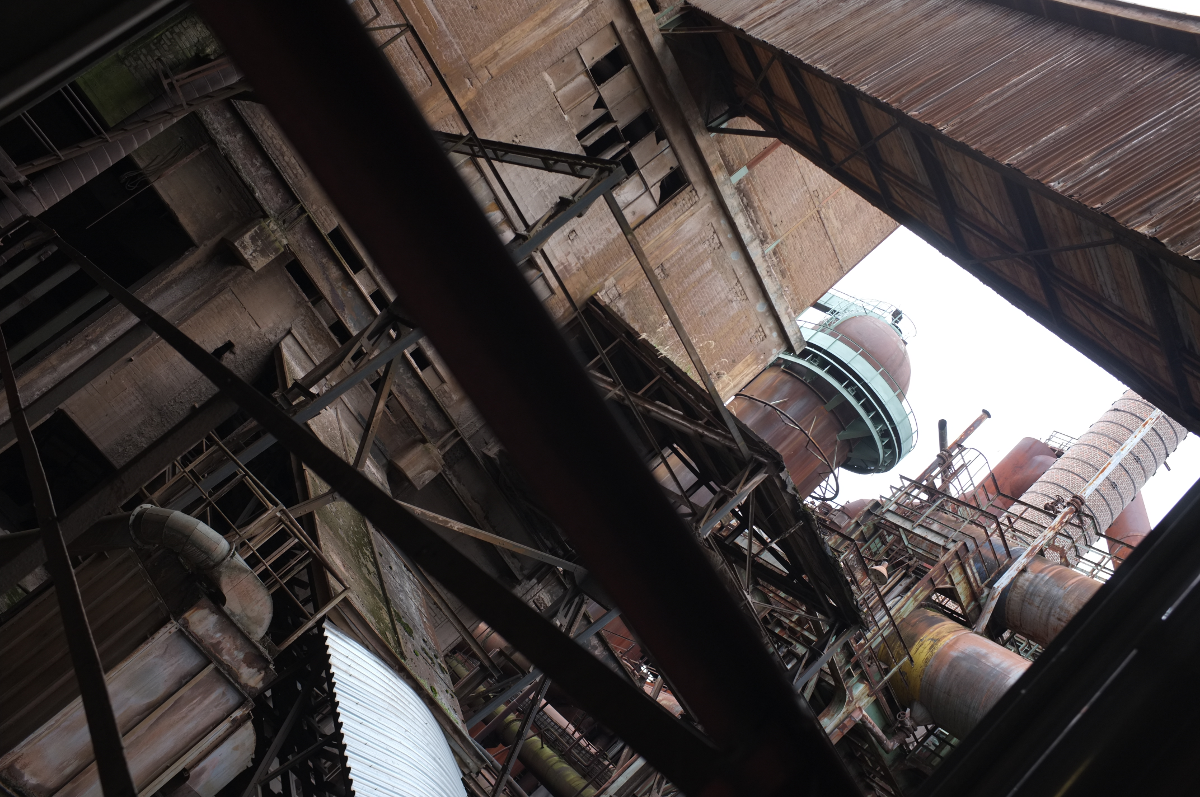
\includegraphics[width=0.7\textwidth]{Examples/example_5.png}
  \caption{Erstes Bild, Völklinger Hütte}
  \label{fig:Huette}
\end{figure}


\subsection{Wrapfigure}
Abbildung~\ref{fig:Huette} ist zwar ganz nett anzusehen, aber vielleicht sähe es eleganter aus, wenn die Abbildung 
von unserem Textabschnitt umflossen werden würde. Diese Art von Abbildungen sollte jedoch sparsam und mit großer Sorgfalt eingesetzt werden, da es zu unschönen Darstellungen kommen kann.
\blindtext
\begin{wrapfigure}{l}{0.4\textwidth}
  \centering
  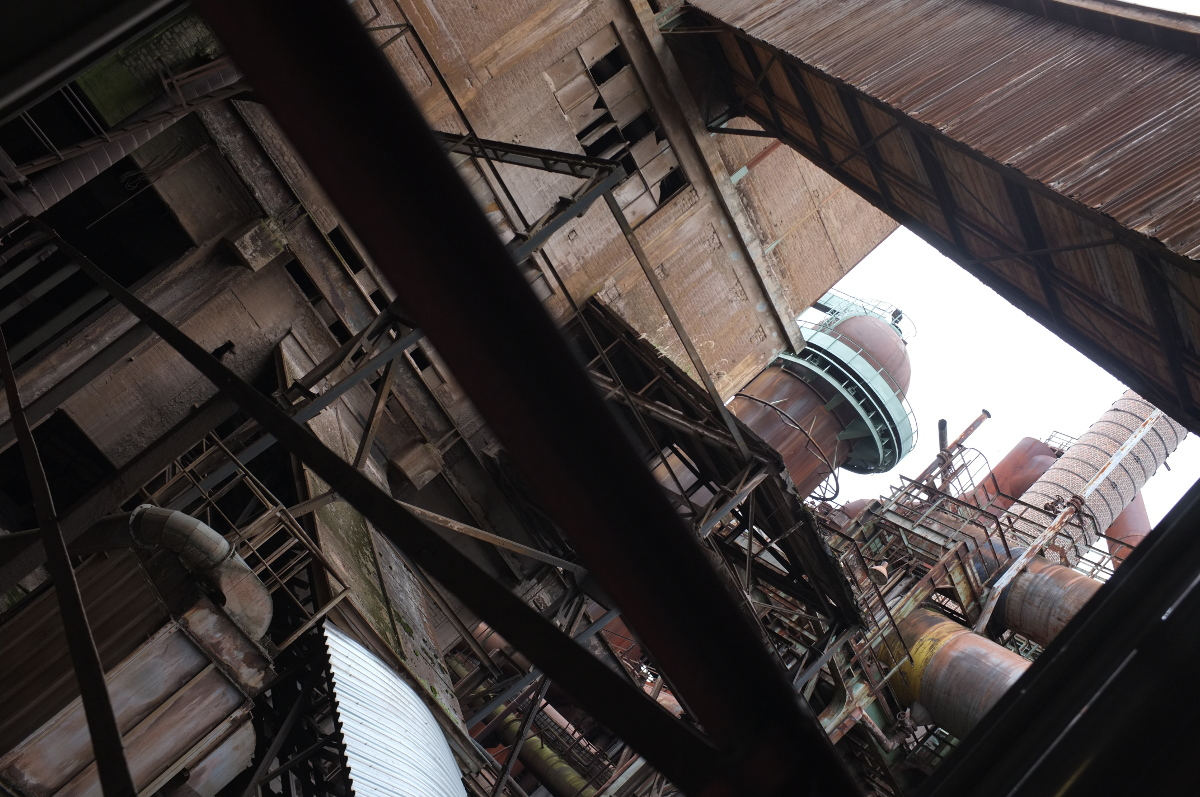
\includegraphics[width=0.4\textwidth]{Examples/example_5.jpg}
  \caption{Völklinger Hütte, *.jpg}
  \label{fig:Huette2}
\end{wrapfigure}
\blindtext


\subsection{Subfigures}
Es ist ebenso möglich, mehrere Abbildungen nebeneinander zu setzen, wie in Abbildung~\ref{fig:Beide} zu sehen ist. Eine separate Referenzierung ist auch möglich: Abbildung~\ref{subfig:abbone}.
\begin{figure}[bth]
  \subfloat[Erstes ...]{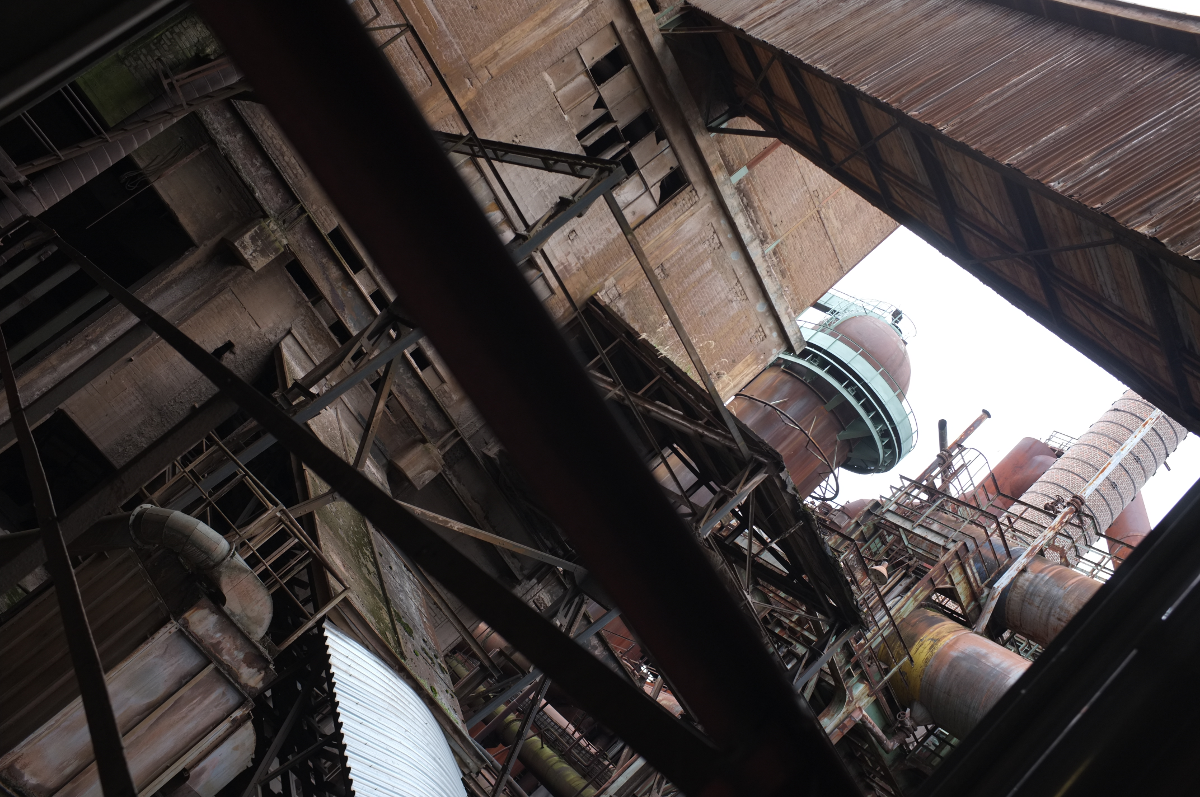
\includegraphics[width=0.49\textwidth]{Examples/example_5.png}\label{subfig:abbone}}\hfill
  \subfloat[... und zweites Bild]{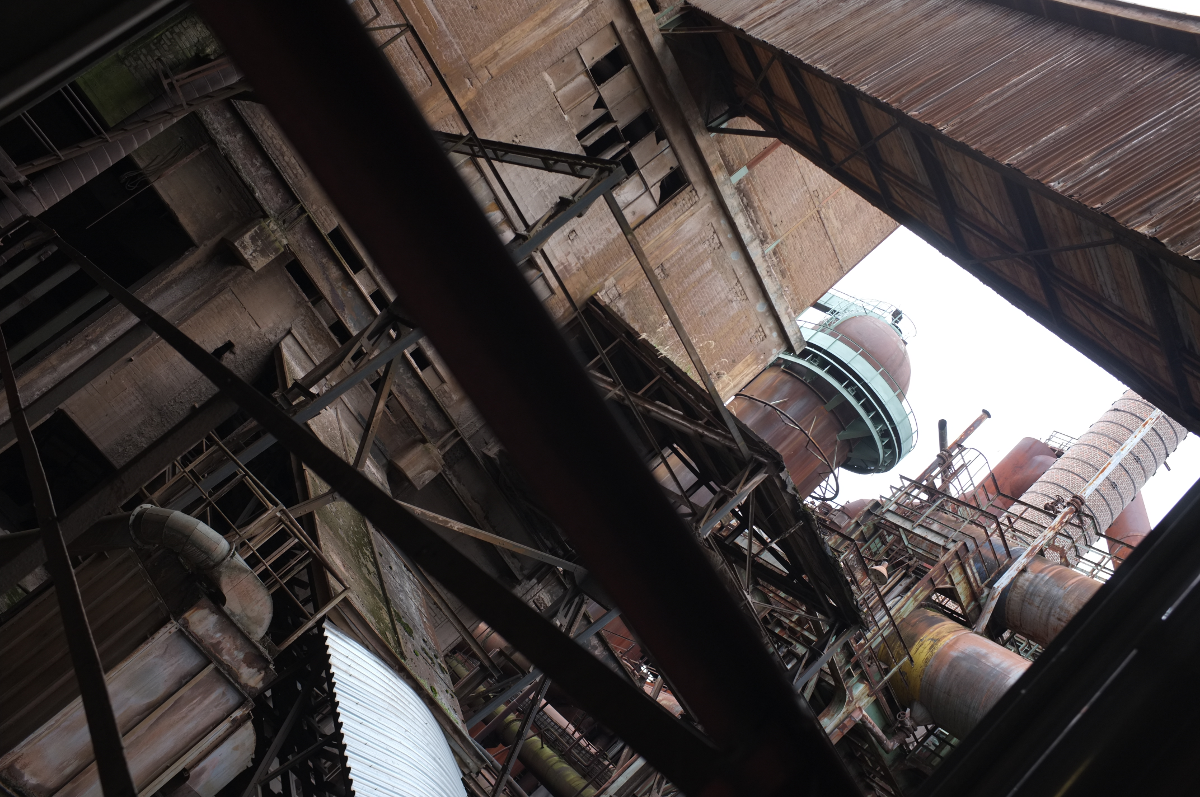
\includegraphics[width=0.49\textwidth]{Examples/example_5.png}\label{subfig:abbtwo}}
  \caption{Mehrere Abbildungen nebeneinander}
  \label{fig:Beide}
\end{figure}


\subsection{Qualitätsunterschiede}
\begin{figure}[p]
	\centering
  \subfloat[\textit{PDF}-Format]{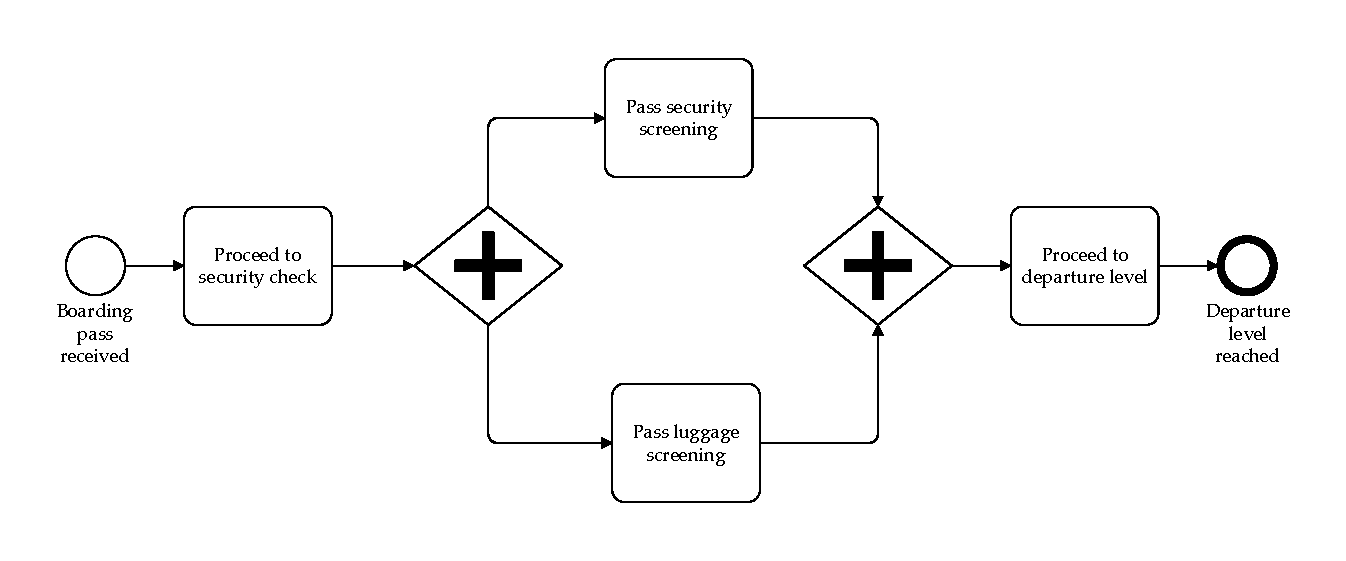
\includegraphics[width=0.65\textwidth]{Examples/bpmn.pdf}} \\
  \subfloat[\textit{JPG}-Format]{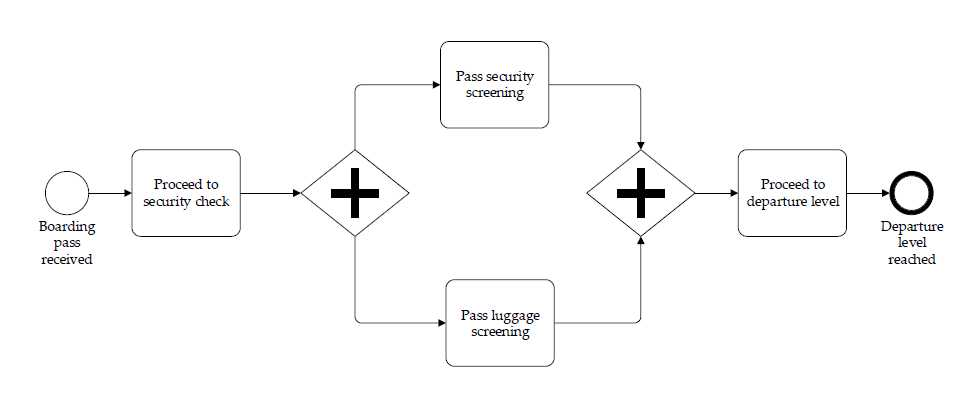
\includegraphics[width=0.65\textwidth]{Examples/bpmn.jpg}}
  \caption{Beide Formate im Vergleich}
  \label{fig:pdfvsjpg}
\end{figure}

\begin{figure}[p]
	\centering
  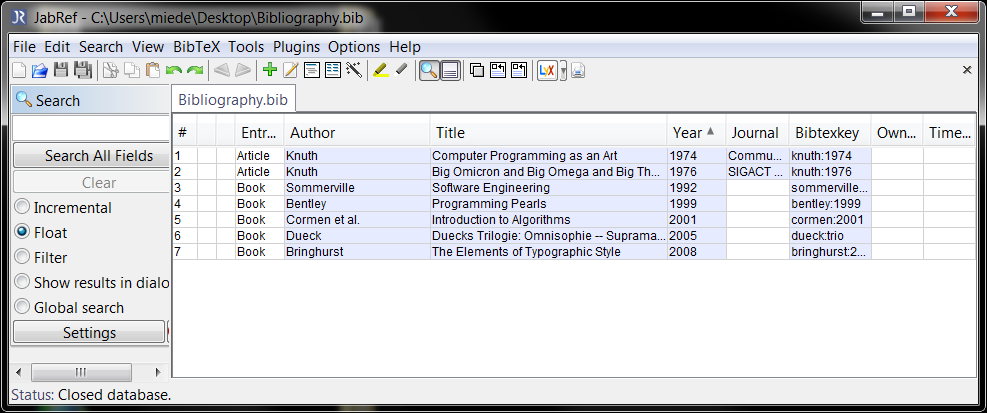
\includegraphics[width=0.65\textwidth]{Examples/jabref.png}
   \caption{\textit{PNG}-Format}
  \label{fig:pngvsjpg1}
\end{figure}

\begin{figure}[p]
	\centering
  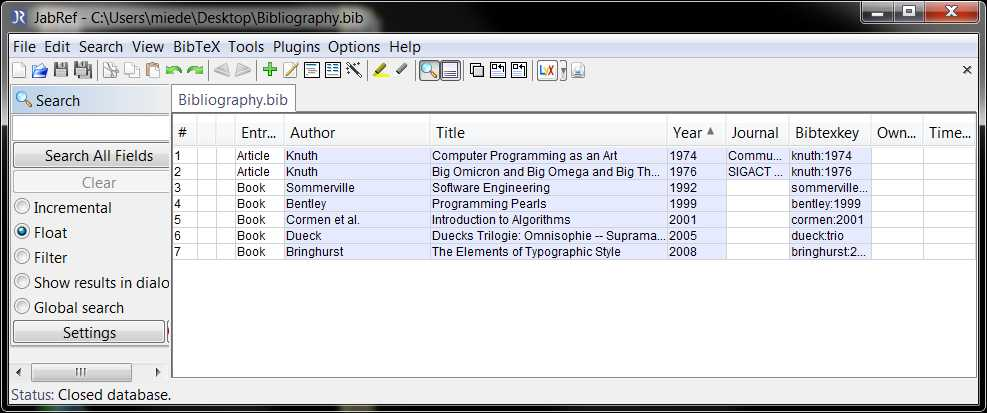
\includegraphics[width=0.65\textwidth]{Examples/jabref.jpg}
   \caption{\textit{JPG}-Format}
  \label{fig:pngvsjpg2}
\end{figure}

Leider haben die unterschiedlichen Grafikformate bedingt durch die unterschiedlichen Kompressionsverfahren einige Schwächen, insbesondere die Umwandlung in das \textit{JPG}-Format erzeugt unangenehme Artefakte im Bild. \autoref{fig:pdfvsjpg} zeigt die Unterschiede zwischen \textit{PDF-Format} und \textit{JPG-Format} im Vergleich. 

Wenn eine \textit{*.pdf}-Datei nicht infrage kommt, beispielsweise bei Screenshots, ist unbedingt das \textit{PNG-Format} vorzuziehen. 
Den Unterschied machen \autoref{fig:pngvsjpg1} und \autoref{fig:pngvsjpg2} deutlich.

"`Faustregeln"' im Umgang mit Abbildungen:
\begin{itemize}
	\item Diagramme bzw. alles, was Linien usw. enthält: \textit{PDF} (im Vektorformat).
	\item Screenshots bzw. alles, was größere gleichfarbige Flächen enthält: \textit{PNG}.
	\item Der Rest (in der Regel Fotos): \textit{JPEG}.
\end{itemize}





%*******************************
% 			Listings 		   *
%*******************************

\section{Quellcode einbinden}
Das Package \textit{lstlisting} ermöglicht es, Quellcode ansprechend in das Dokument einzubinden. Man kann Quellcode einzeilig einbinden 
mittels \lstinline{\lstinline|Quellcode|}. Dabei ist darauf zu achten, dass der Befehl einmal mit \{ \} und einmal mit | | aufgerufen werden kann, je nachdem, 
welche Zeichen im angegebenen Quelltext genutzt werden. 
Es ist auch möglich eine eigene Umgebung für Quelltext zu schaffen:

\begin{lstlisting}[caption=Erstes Listing,style=Java]
private Umgebung(int i, int k)
{
	System.out.println("Eine Funktion mit " + i + "und" + k ".");
}
\end{lstlisting}  

Wer Quelltext aus externen Dateien einbinden möchte, geht wie folgt vor:

\lstinputlisting
[caption={Externer Quellcode},style=Java]
{Examples/Code.java}

Wie genau der Quellcode formatiert und gefärbt ist, ist in \textit{htwsaar.i.mst.config.tex} hinterlegt, wobei fü verschiedene Sprachen auch eigene Styles angelegt werden
können (hier z.B. für Java).
\section{Mathematische Ausdrücke}
Mathematische Ausdrücke sind eine kleine Kunst für sich. Am allereinfachsten kann man eine Formel, wie \(a + b = c\) in den Fließtext einbinden, wobei LaTeX die Höhe der Ausdrücke der Zeile anpasst,
wie hier zu sehen \(\sum_{y=0}^{x} a\) . In einer Umgebung sieht das schon anders aus:
\begin{equation}
  \sum_{y=0}^{x} a
\end{equation}

Griechische Buchstaben:
\begin{equation}
	\alpha\beta\gamma\delta\epsilon\varepsilon\zeta\eta
	\theta\iota\kappa\lambda\mu\nu\xi\pi\varpi\rho\varrho
	\sigma\tau\upsilon\phi\varphi\chi\psi\omega
\end{equation}

Brüche:
\begin{equation}
	Ergebnis = \frac{a}{b}
\end{equation}

\begin{equation}
	\frac{\sin{\alpha}^2 + \cos{\alpha}^2}{1} = 1
\end{equation}

\begin{equation}
	\frac{-9x}{\frac{2y}{3z+2}}
\end{equation}

Text innerhalb von Formeln:
\begin{equation}
\sum_{y=1}^{n} y = \frac{n*(n+1)}{2}
\quad
\text{Gaußsche Summenformel}
\end{equation}

Hoch- bzw. Tiefstellungen:
\begin{equation}
	x_{i,j}^2
\end{equation}

\begin{equation}
	{x_{i,j}}^2
\end{equation}

\begin{equation}
	x_{n_0}
\end{equation}


Matrizen:
Matrizen werden innerhalb der mathematischen Umgebung als wiederum neue Umgebung eingebunden. Wie bei Tabellen auch werden Zeilen durch \lstinline{\\} und Spalten durch \lstinline{&} getrennt.

\begin{equation}
	\begin{pmatrix} 
		a&b\\
		c&d 
	\end{pmatrix}
\end{equation} 

\begin{equation}
	\begin{vmatrix} 
		a&b\\
		c&d 
	\end{vmatrix}
\end{equation} 

Fallunterscheidung:
\begin{equation}
	f(x) = 
	\begin{cases}
		0, &\text{falls } x < 0 \\
		1, &\text{falls } x \geq 0
	\end{cases}
\end{equation}




%############################################################
\clearpage\section{To-Do-Notes}
Um bei einer längeren Arbeit nicht den Überblick zu verlieren, an welcher Stelle es nötig ist
weiter zu arbeiten, bietet es sich an, kleine Notizen einzufügen. Das Package \textit{todonotes}
stellt eine elegante Lösung bereit, um differenziert und vielfarbig jene Abschnitte zu kennzeichnen,
die einer weiteren Bearbeitung bedürfen.

\subsection*{Beispiel für To-Do-Notes}
Dies hier ist ein Blindtext zum Testen von Textausgaben. Wer diesen Text liest, ist selbst
\todo{Plain todonotes.} schuld. Der Text gibt lediglich den Grauwert der Schrift an. Ist das wirklich so? Ist es
gleichgültig, ob ich schreibe: Dies ist ein Blindtext? oder Huardest gefburn? Kjift?
mitnichten! Ein Blindtext bietet mir wichtige Informationen. An ihm messe ich die Les-
barkeit einer Schrift, ihre Anmutung, \todo{Plain todonotes.}wie harmonisch die Figuren zueinander stehen
und prüfe, wie breit oder schmal sie läuft. Ein Blindtext sollte möglichst viele verschie-
dene Buchstaben enthalten und in der Originalsprache gesetzt sein. Er muss keinen
Sinn ergeben, sollte aber lesbar sein.\todo[nolist]{Todonote that is only shown in the margin and not in
the list of todos.}%
Fremdsprachige Texte wie Lorem ipsum dienen
nicht dem eigentlichen Zweck, da sie eine falsche Anmutung vermitteln. Dies hier ist
ein Blindtext zum Testen von Textausgaben. Wer diesen Text liest, ist selbst schuld. 

\todo[inline]{A very long todonote that certainly will fill more
than a single line in the list of todos. Just to make sure let's add
some more text \ldots}

Der Text gibt lediglich den Grauwert der Schrift an. Ist das wirklich so? Ist es gleichgültig,
ob ich schreibe: Dies ist ein Blindtext? oder Huardest gefburn? Kjift? mitnichten!
\todo[noline]{A note with no line back to the text.}
Ein Blindtext bietet mir wichtige Informationen. An ihm messe ich die Lesbarkeit einer
Schrift, ihre Anmutung, wie harmonisch die Figuren zueinander stehen und prüfe, wie
\todo[caption={A short entry in the list of todos}]{A very long
todonote that certainly will fill more than a single line in the
list of todos \ldots}
breit oder schmal sie läuft. Ein Blindtext sollte möglichst viele verschiedene Buchstaben
enthalten und in der Originalsprache gesetzt sein. Er muss keinen Sinn ergeben, sollte
aber lesbar sein. Fremdsprachige Texte wie Lorem ipsum dienen nicht dem eigentlichen Zweck, 
da sie eine falsche Anmutung vermitteln.
\missingfigure{A figure I have to make \ldots}

%Nummerierte ToDo-Notes
\todox{Erste Nummer...}
\todox{Zweite Nummer...}

%Alles To-Dos als Liste ausgegeben
Nachfolgend wird noch eine Liste aller To-Dos auf einer separaten 
Seite ausgegeben.
%\begingroup
	%\let\clearpage\relax
	%\let\cleardoublepage\relax
	\listoftodos
%\endgroup 


 		% Abschlussarbeit geht!
%\cleardoublepage\include{Chapters/KapitelBachelorarbeit} % <<< Hier alle Chapter der Abschlussarbeit (einzeln) einbinden

%********************************************************************
% Bibliography/References
%*******************************************************
\cleardoublepage%********************************************************************
% Bibliography
%*******************************************************
\printbibliography

%********************************************************************
% List of Figures etc.
%*******************************************************
\cleardoublepage%*******************************************************
% Verzeichnisse (Abbildungen, Tabellen, Listings, etc.)
%*******************************************************
\cleardoublepage
\begingroup
	\let\clearpage\relax
	\let\cleardoublepage\relax
	\listoffigures
	\listoftables
	%\addcontentsline{toc}{chapter}{\lstlistlistingname}
	\lstlistoflistings 
\endgroup 
%*******************************************************
% Abkürzungsverzeichnis
%*******************************************************
\chapter*{Abkürzungsverzeichnis}
\markboth{Abkürzungsverzeichnis}{}
\addcontentsline{toc}{chapter}{Abkürzungsverzeichnis}	
	%Hier alle benötigten Abkürzungen einfügen
	\begin{acronym}[WLAN] % LONGEST ACRONYM HERE FOR CORRECT SPACING
	    \acro{WLAN}{Wireless Local Area Network}
	    \acro{TCP}{Transmission Control Protocol}
	    \acro{GoF}{Gang of Four}
	\end{acronym}
	
	

% ********************************************************************
% Appendix/Anhang
%***************************************************************
\appendix
\part*{Anhang}
\cleardoublepage%********************************************************************
% Appendix
%*******************************************************
\chapter{Erster Abschnitt des Anhangs}
In den Anhang gehören "`Hintergrundinformationen"', also weiterführende Information, ausführliche Listings, Graphen, Diagramme oder Tabellen, die den Haupttext mit detaillierten Informationen ergänzen. 

\blindtext
\blindtext
\blindtext



%*******************************************************
\cleardoublepage\pagestyle{empty}

\hfill

\vfill


\pdfbookmark[0]{Kolophon}{colophon}
\section*{Kolophon}
Dieses Dokument wurde mit der \LaTeX-Vorlage für Abschlussarbeiten an der htw saar im Bereich Informatik/Mechatronik-Sensortechnik erstellt (\currentVersion). Die Vorlage wurde von Yves Hary und Andr\'e Miede entwickelt (mit freundlicher Unterstützung von Thomas Kretschmer, Helmut G. Folz und Martina Lehser). Daten: (F)\makeatletter\f@size\makeatother\ -- (B)\the\textwidth\ -- (H)\the\textheight\ 


\end{document}
% ********************************************************************
